% =============================================================================
%  三、问题求解（三）：随机过程重构
% =============================================================================
\subsection{方法替换：随机过程的重构与求解}

\subsubsection{状态空间与协变量}

替换方法的第一步是把“层级”从标签变成状态。本文取第二节定义的分位带层级
$S_i\in\{1,\dots,5\}$ 为状态空间：$1$ 为最高效层（类内效率前 10\%），$5$ 为
最低效层（后 45\%）。选择分位带而非剔除式的理由已在复现部分的敏感性讨论中说明：
状态空间必须被占满、层规模必须稳定，否则强度无法估计。

协变量取五个维度，均由 14 个题项合成并标准化：
\begin{equation}
\bz_i=\bigl(z_{i1},\dots,z_{i5}\bigr)^{\top}\in\R^{5},
\label{eq:cov}
\end{equation}
其中 $z_{i1}$ 为复习巩固、$z_{i2}$ 为应试训练、$z_{i3}$ 为输入训练、$z_{i4}$
为心理作息、$z_{i5}$ 为兴趣拓展。复习巩固由复习、辅导、课外合成，应试训练由
考试次数、模拟考合成，输入训练由背诵、听力、口语、阅读合成，心理作息由心
理、休息合成，兴趣拓展由兴趣、课外、出国意愿合成。五者恰好对应原文的四个
投入维度并做了更细的拆分，好处是后文的“动作”可以直接挂在这些维度上。

\subsubsection{生灭过程的设定}

设 $S_t$ 为学生在学期内第 $t$ 周所处的层级，$t$ 以周为单位连续取值。假设
$S_t$ 是状态空间 $\{1,\dots,5\}$ 上的生灭过程：只允许相邻转移，$1$ 与 $5$
为反射壁（不能越界），且转移强度只依赖于当前状态与个体协变量：
\begin{equation}
\lambda_i=\frac{c\,\rho_i}{1+\rho_i},\qquad
\mu_i=\frac{c}{1+\rho_i},\qquad
\rho_i=\exp\bigl(\alpha+\bdelta^{\top}\bz_i\bigr),
\label{eq:bd}
\end{equation}
其中 $\lambda_i$ 为上行强度（$k\to k-1$），$\mu_i$ 为下行强度（$k\to
k+1$）。这一参数化的要点是：\textbf{上行与下行强度之比恰为 $\rho_i$}，
\begin{equation}
\frac{\lambda_i}{\mu_i}=\rho_i ,
\label{eq:ratio}
\end{equation}
而 $\lambda_i+\mu_i=c$ 对所有个体相同。于是 $\rho_i$ 有了清晰的解释：它是
“改善与恶化”的相对速率，$\rho_i>1$ 表示净漂移向上，$\rho_i<1$ 表示净漂移
向下；$c$ 是时间尺度，决定“事件发生得多快”。把“方向”与“速度”解耦，是这
一参数化相对“分别估计 $\lambda,\mu$”的最大好处：方向由协变量解释，速度由
一个标量统一控制。

生成矩阵为
\begin{equation}
\bQ_i=\begin{pmatrix}
-\mu_i & \mu_i & 0 & 0 & 0\\
\lambda_i & -(\lambda_i+\mu_i) & \mu_i & 0 & 0\\
0 & \lambda_i & -(\lambda_i+\mu_i) & \mu_i & 0\\
0 & 0 & \lambda_i & -(\lambda_i+\mu_i) & \mu_i\\
0 & 0 & 0 & \lambda_i & -\lambda_i
\end{pmatrix},
\label{eq:Q}
\end{equation}
转移概率矩阵为 $\bP_i(t)=\exp(\bQ_i t)=\sum_{m\ge0}(\bQ_i t)^m/m!$，用
Padé 近似数值计算。

\subsubsection{一致化、嵌入链与谱隙}

生灭过程只是名字，要让它成为可计算的对象，必须落到具体的构造。注意
$\lambda_i+\mu_i=c$ 与状态无关，这一巧合正是 Poisson 过程与连续时间链之间的桥梁：
可以把状态轨道“打散”成两层随机性——一条速率为 $c$ 的 Poisson 事件流
$N(t)$，每次事件以概率 $p_i=\rho_i/(1+\rho_i)$ 上行、以 $1-p_i$ 下行。于是
\begin{equation}
\bP_i(t)=\sum_{n\ge0}e^{-ct}\frac{(ct)^{n}}{n!}\bigl(\bP_i^{J}\bigr)^{n},
\qquad \bP_i^{J}=\bm{I}+\frac{1}{c}\bQ_i ,
\label{eq:uni}
\end{equation}
其中 $\bP_i^{J}$ 称为嵌入链（跳链）的转移矩阵。式\eqref{eq:uni} 是
“Poisson 计数 + 离散跳链”的加权和，与 $\exp(\bQ_i t)$ 在数学上恒等：
用 400 项截断重建 $\bP_{480}(16)$，与矩阵指数解的最大绝对误差为
$3.8\times10^{-15}$，说明两种语言描述的是同一个对象。

这条式子的用处不只是验算。$c=2.54$ 周$^{-1}$ 意味着学生平均每 $0.39$ 周
就有一次“足以改变层级”的行为波动，一个学期（16 周）内期望发生
$40.6$ 次状态试探，而 16 周内一次试探都没有的概率是
$e^{-40.6}=2.2\times10^{-18}$。换言之，\textbf{“周”这个观测尺度相对于过程
本身是慢的}：我们看到的是四十余次往返之后的净位置，而不是一次跳跃的结果。

嵌入链与连续链的平稳分布完全相同（五类的数值差均在 $10^{-15}$ 量级），
因为 $\lambda+\mu$ 恒定使均匀化不改变相对权重。五个状态互通且状态数有限，
由有限状态马尔可夫链的判别法，五个状态全是正常返，不存在非常返类，故平稳分布唯一
且同时是极限分布。

极限定理除了“收敛”，还给出\textbf{收敛速度}。以 S480 为例，$\bQ$ 的特征值
为 $0,-0.5165,-1.7669,-3.3126,-4.5630$；谱隙 $|\lambda_2|$ 给出
$\|\bP(t)-\bpi\|_{\mathrm{TV}}\le C e^{-|\lambda_2|t}$。五类的谱隙在
$0.497$--$0.545$ 之间，对应半衰期 $1.27$--$1.39$ 周、到 $1\%$ 总变差距离
需 $8.4$--$9.3$ 周（表 \ref{tab:spectrum}）。这为“16 周已基本混合”提供了
严格的速度：五类在 16 周时的总变差距离只有 $1.7\times10^{-4}$--
$2.8\times10^{-4}$。也就解释了为什么“一次跃层”的收益是一次性的——过程在
半个学期内就把初始位置的信息忘干净了。

\begin{table}[H]
\centering
\tabfont
\caption{五类的谱隙、混合时间与 16 周时的总变差距离}
\label{tab:spectrum}
\begin{tabular}{@{}lccccc@{}}
\toprule
类 & $\rho$（中位） & $\lambda_2$ & 半衰期（周） & $1\%$ 混合（周） & 16 周总变差 \\
\midrule
1 & 0.805 & $-0.497$ & 1.39 & 9.26 & $2.8\times10^{-4}$ \\
2 & 0.612 & $-0.545$ & 1.27 & 8.45 & $1.7\times10^{-4}$ \\
3 & 0.713 & $-0.514$ & 1.35 & 8.96 & $2.4\times10^{-4}$ \\
4 & 0.653 & $-0.531$ & 1.31 & 8.68 & $2.0\times10^{-4}$ \\
5 & 0.669 & $-0.526$ & 1.32 & 8.76 & $2.1\times10^{-4}$ \\
\bottomrule
\end{tabular}

\vspace{2pt}
\parbox{\textwidth}{\tabfont 注：$\rho$ 取类内中位数作为该类代表；$\lambda_2$
为 $\bQ$ 的第二大特征值；混合时间按 $\ln(1/0.01)/|\lambda_2|$ 计算。}
\end{table}

把“上行”单独看成计数过程，还可读出比概率更细的结构：由 Poisson 的稀疏性，
第 $k$ 层出发的上行事件数 $N_k(t)\sim\text{Pois}(\lambda_k t)$，等待时间
$\tau_k\sim\text{Exp}(\lambda_k)$，
\begin{equation}
\Pbb(N_k(t)=m)=e^{-\lambda_k t}\frac{(\lambda_k t)^m}{m!},
\qquad
\Pbb(\tau_k>t)=e^{-\lambda_k t}.
\label{eq:pois}
\end{equation}
对 S480 在第 5 层，$\lambda_5=1.049$ 周$^{-1}$：平均 $0.954$ 周上行一次，
中位等待 $0.661$ 周，16 周内上行事件的期望次数达 $16.8$ 次。这里必须澄清
一个口径：前文与表 \ref{tab:s480} 所说的“16 周跃层概率 $0.642$”，指的是
\textbf{16 周末不在第 5 层}的概率（净位移），而不是“期间从未跃层”的概率；
后者是 $e^{-\lambda_5 T}\approx5\times10^{-8}$。两个口径相差五个数量级，恰恰
说明原文式“单步提升”的问题所在：过程是高频往返，净位移只是往返的差，
不是一次冲刺的成果。

\subsubsection{平稳分布与“下行锁定”}

对式\eqref{eq:Q} 的链，细致平衡给出 $\pi_{k-1}\mu_i=\pi_k\lambda_i$，即
$\pi_k=\pi_{k-1}/\rho_i$。归一化后
\begin{equation}
\pi_{i,k}=\frac{r_i^{\,k-1}\,(r_i-1)}{r_i^{5}-1},\qquad r_i=\frac{1}{\rho_i},
\quad k=1,\dots,5 .
\label{eq:pi}
\end{equation}
当 $\rho_i<1$（即 $r_i>1$）时，$\pi$ 随 $k$ 递增，长期停留在第 5 层的概率
最大；当 $\rho_i>1$ 时相反。这一条式子把“效率会不会自己变好”这个问题变成
了一个参数符号问题。

估计结果见表 \ref{tab:ctmcpar}。$\alpha=-0.382$（标准误 0.035），五个
$\delta$ 中只有“兴趣拓展”为正（0.305，标准误 0.097），其余四项均为负，
其中“心理作息”最负（$-0.272$）。由于 $\rho_i=\exp(\alpha+\bdelta^{\top}z)$
的中位数只有 0.682，\textbf{98.1\% 的学生满足 $\rho_i<1$}，即绝大多数人的
净漂移向下。这一结果与截面观测高度一致：观测到 45.1\% 的学生位于第 5 层，
而模型给出的平稳分布同样把最大质量放在第 5 层（表 \ref{tab:stationary}）。

“为什么多数人漂移向下”需要谨慎解释。在 DEA 口径下，效率是“产出/投入”的
相对比值，\textbf{增加投入而产出不变，效率就会下降}。因此 $\delta_{\text{复习}}<0$、
$\delta_{\text{作息}}<0$ 并不意味着“复习与休息有害”，而是意味着“在效率这
把尺子上，单纯加时间会稀释比值”。这一点是本文与原文最重要的分歧：原文把
“向高效同伴学习更多投入”当作改进路径，而随机过程模型给出的参数显示，这样
做在效率口径上反而使 $\rho$ 下降。后文的策略优化会进一步放大这一分歧。

\begin{table}[htbp]
\centering
\tabfont
\caption{生灭过程参数估计（$\rho_i=\exp(\alpha+\bdelta^{\top}\bz_i)$，BFGS 极大似然）}
\label{tab:ctmcpar}
\begin{tabular}{@{}lccc@{}}
\toprule
变量 & 估计值 & 标准误 & $\exp(\hat\delta_j)$ \\
\midrule
常数项 $\alpha$ & $-0.382$ & 0.035 & 0.683 \\
复习巩固 & $-0.135$ & 0.063 & 0.873 \\
应试训练 & $-0.075$ & 0.040 & 0.928 \\
输入训练 & $0.003$ & 0.096 & 1.003 \\
心理作息 & $-0.272$ & 0.056 & 0.762 \\
兴趣拓展 & $0.305$ & 0.097 & 1.357 \\
\bottomrule
\end{tabular}
\end{table}

\subsubsection{极大似然估计与识别性}

由于没有纵向面板，本文采用“截面边际似然”：把个体 $i$ 观测到的层级 $S_i$
视为其在自身平稳分布 $\pi_i$ 下的一次抽样，构造
\begin{equation}
\ell(\alpha,\bdelta)=\sum_{i=1}^{n}\log\pi_{i,S_i}
=\sum_{i=1}^{n}\Bigl[(S_i-1)\log r_i+\log(r_i-1)-\log(r_i^5-1)\Bigr],
\label{eq:lik}
\end{equation}
用 BFGS 极大化，标准误由观测信息阵（数值 Hessian 的逆）给出。这一似然只
使用截面信息，因此\textbf{只能识别 $\rho$ 的相对大小与符号，不能识别绝对
时间尺度}；后者由 3.3.5 节的时间标定给出。这是本文在方法论上必须承认的
边界，而不是可以绕过的技术细节。

拟合诊断见表 \ref{tab:stationary}：模型期望的层分布与观测相比，第 1、2 层
略低、第 3、4 层偏高、第 5 层偏低（观测 45.1\% 对模型 37.3\%），
$\chi^2=34.61$（$df=4$，$p\approx1.5\times10^{-7}$），分类准确率仅
45.7\%。这些数字不好看，但它们说明了一件重要的事：\textbf{截面似然只能
刻画“群体层面的漂移方向”，无法预测个体的具体层级}。这也解释了为什么模型
的价值不在“预测谁在第几层”，而在“给出转移强度、时间尺度与动作的相对效
应”——后三者才是原文完全缺失的。

\begin{table}[htbp]
\centering
\tabfont
\caption{平稳分布与观测分布的对照（拟合诊断）}
\label{tab:stationary}
\begin{tabular}{@{}lcccccc@{}}
\toprule
层级 & L1 & L2 & L3 & L4 & L5 & 检验 \\
\midrule
观测人数 & 55 & 76 & 77 & 77 & 234 & \\
观测比例 & 0.106 & 0.146 & 0.148 & 0.148 & 0.451 & \\
模型期望人数 & 47 & 63 & 88 & 128 & 193 & $\chi^2=34.61$ \\
模型期望比例 & 0.090 & 0.121 & 0.170 & 0.247 & 0.373 & $p\approx1.5\times10^{-7}$ \\
\bottomrule
\end{tabular}

\vspace{2pt}
\parbox{\textwidth}{\tabfont 注：模型期望人数按四舍五入取整显示；$\chi^2$ 检验使用未舍入的期望频数。}
\end{table}

\begin{figure}[htbp]
\centering
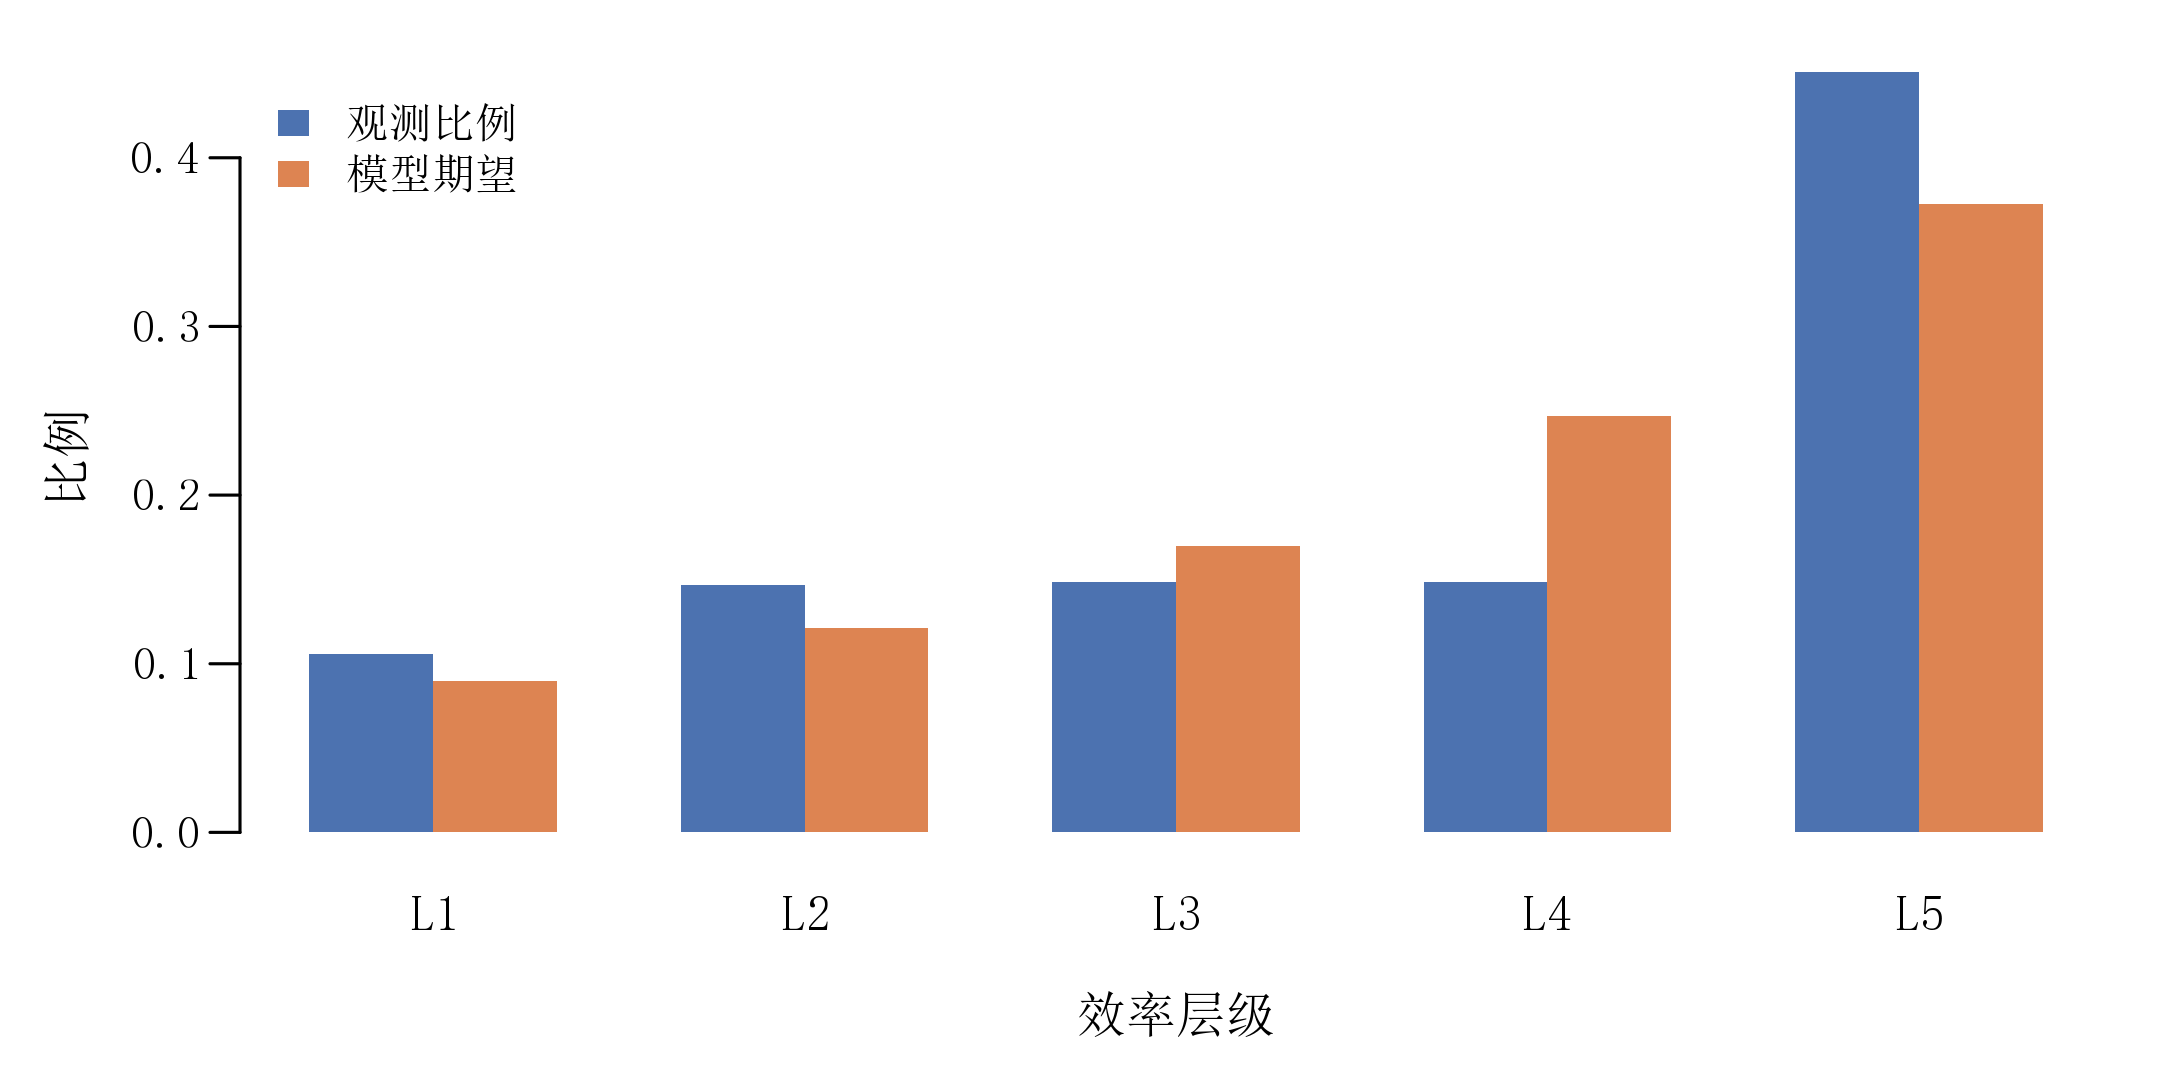
\includegraphics[width=0.78\textwidth]{fig_stationary}
\caption{观测层级比例与模型平稳分布的对比}
\label{fig:stationary}
\end{figure}

\subsubsection{时间标定与首达时间}

式\eqref{eq:bd} 中的 $c$ 是唯一无法由截面数据识别的参数。本文用原文的时
间锚点标定它：原文报告 S480 在一个学期（16 周）内完成一次跃层、效率提升
25.38\%，本文取“第 5 类的中位个体在一个学期内完成一次跃层”为标定条件，解
得
\begin{equation}
c=2.54\ \text{周}^{-1},
\label{eq:c}
\end{equation}
即平均每 0.39 周发生一次层级转移事件（上行或下行）。取 S480 的
$\rho=0.703$，则 $\lambda=1.048$ 周$^{-1}$、$\mu=1.491$ 周$^{-1}$，下行比
上行快 42\%。

首达时间 $T_1=\inf\{t:S_t=1\}$ 的期望 $m_k=\E_k[T_1]$ 满足三对角方程组
\begin{equation}
\begin{cases}
m_1=0,\\
\lambda_k\bigl(m_k-m_{k-1}\bigr)+\mu_k\bigl(m_k-m_{k+1}\bigr)=1, & k=2,3,4,\\
\lambda_5\bigl(m_5-m_4\bigr)=1, & k=5\ (\text{反射壁}),
\end{cases}
\label{eq:hitting}
\end{equation}
即“流出速率乘以停留时间等于 1”。这是生灭过程首达时间的标准方程，可直接
写成 $4\times4$ 线性方程组求解，无需模拟。

\begin{table}[htbp]
\centering
\tabfont
\caption{首达时间的解析解与 Gillespie 模拟校验（1000 条路径）}
\label{tab:mc}
\begin{tabular}{@{}lcccccc@{}}
\toprule
个体 & 起始层 & $\rho$ & 解析 $m_k$（周） & 模拟均值（周） & 相对误差 \\
\midrule
S480 & 5 & 0.703 & 14.48 & 14.50 & 0.1\% \\
S477 & 4 & 0.669 & 15.04 & 14.48 & 3.7\% \\
S456 & 3 & 0.781 & 8.92 & 8.91 & 0.1\% \\
S494 & 2 & 0.702 & 7.02 & 7.39 & 5.3\% \\
S293 & 1 & 0.880 & 0 & --- & --- \\
\bottomrule
\end{tabular}
\end{table}

校验结果见表 \ref{tab:mc} 与图 \ref{fig:hitting}。五条路径中三条的相对
误差在 0.1\% 量级，另两条分别为 3.7\% 与 5.3\%，后者来自重尾分布下 1000 条
路径的均值估计误差（首达时间的分布右偏严重，少量长路径会显著拉动均值）。
整体上，解析解与模拟一致，说明式\eqref{eq:Q} 与式\eqref{eq:hitting} 的实现
无误。

\begin{figure}[htbp]
\centering
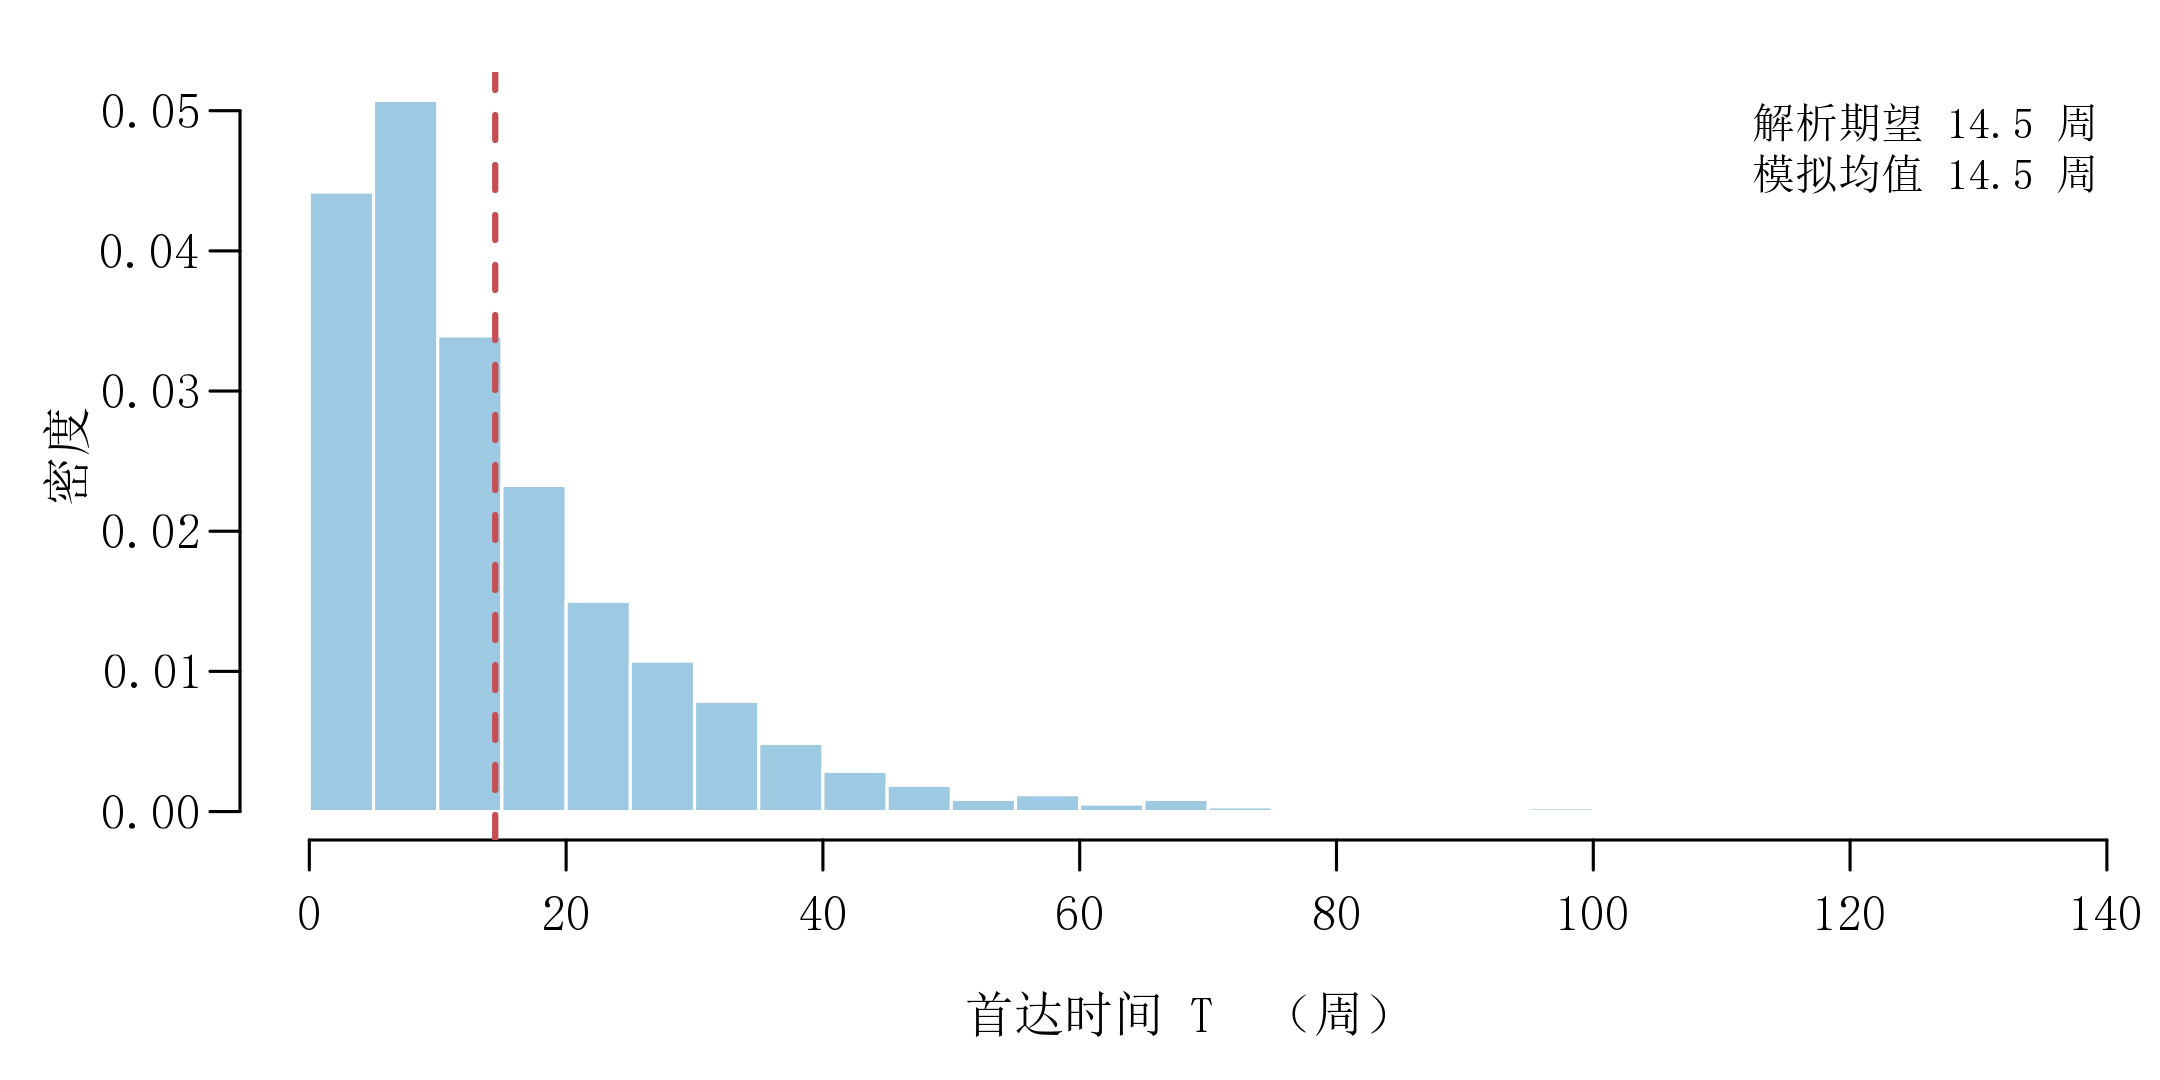
\includegraphics[width=0.78\textwidth]{fig_hitting}
\caption{S480 首达时间的蒙特卡洛分布（直方图）与解析期望（红色虚线）}
\label{fig:hitting}
\end{figure}

\begin{figure}[htbp]
\centering
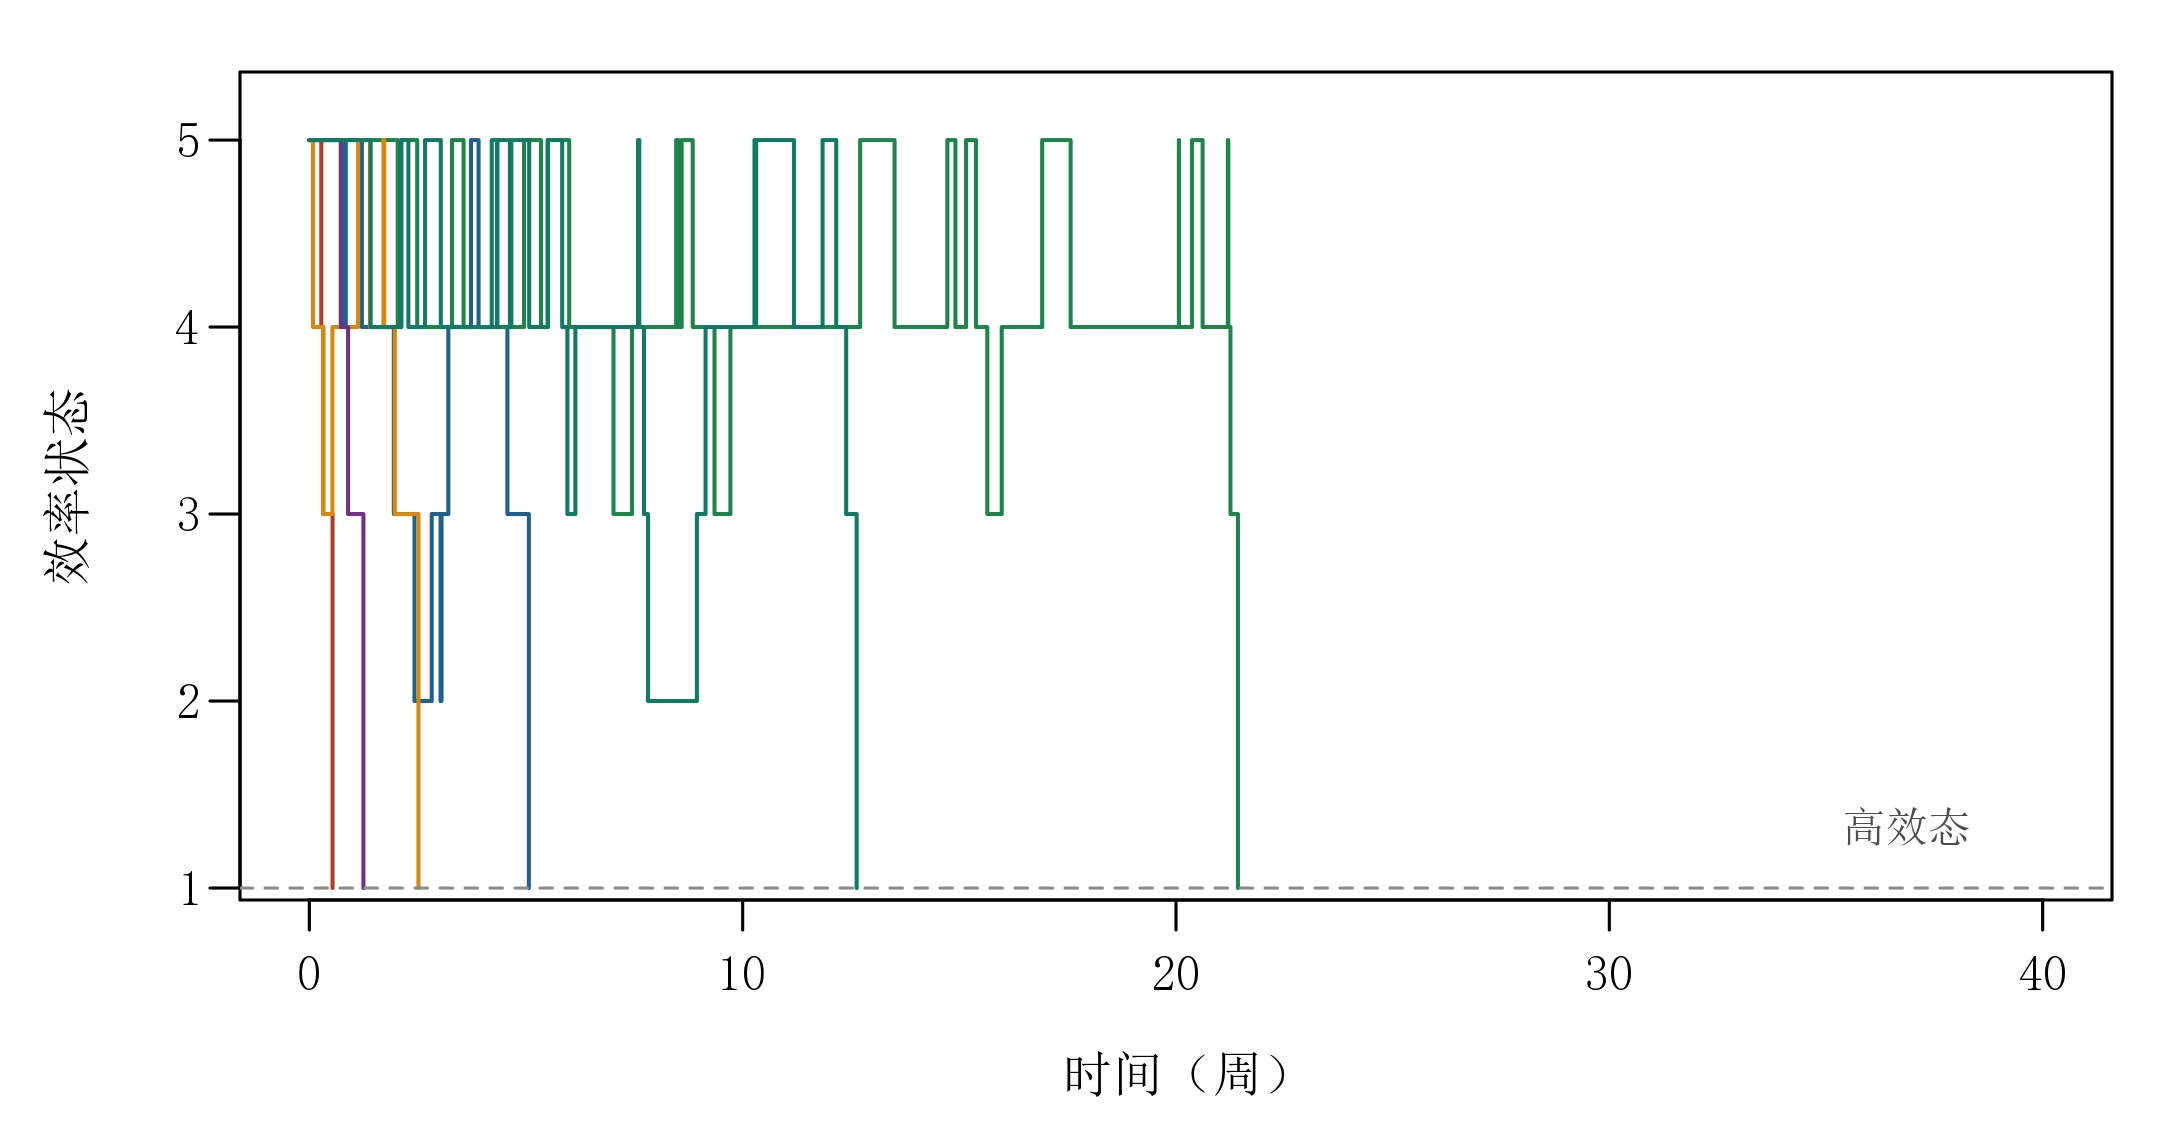
\includegraphics[width=0.85\textwidth]{fig_traj}
\caption{六条独立的生灭过程样本轨道（纵轴为层级，横轴为周）}
\label{fig:traj}
\end{figure}

图 \ref{fig:traj} 给出六条样本轨道。可以看到两个特征：其一，轨道呈“阶梯
状”，在两层之间停留数周才跳一次，这与“学习习惯的改变需要时间”的直觉一致；
其二，多数轨道在 10—20 周内落到第 1 层后便长时间停留，偶有回落到第 2 层。
这一“到达—停留—偶发回落”的形态正是生灭过程与静态排序最直观的区别：静
态排序只说“你在第几层”，生灭过程说“你会在这层待多久、多久掉一次”。

\subsubsection{首达时间的鞅解释与“先到哪一层”}\label{sec:mart}

式\eqref{eq:hitting} 的三对角方程组来自“全期望公式 + 无穷小 $\dd t$”，
推导干净但要一步步做。鞅的停时定理可以一步到位，还顺带给出原文完全
没有的一个量。

\textbf{（1）为什么 $\E[T_1]=m(S_0)$。} 记 $m$ 为 Poisson 方程
$\bQ_i m=-\bm{1}$、$m(1)=0$ 的解（即式\eqref{eq:hitting}）。由 Markov 性，
\begin{equation}
\E\bigl[m(S_{t+\dd t})-m(S_t)\,\big|\,\mathcal{F}_t\bigr]
=\bigl(\bQ_i m\bigr)(S_t)\,\dd t+o(\dd t)=-\dd t+o(\dd t),
\end{equation}
故 $M_t=m(S_t)+t$ 是鞅。状态数有限、$\E[T_1]<\infty$，故
$\{M_{t\wedge T_1}\}$ 一致可积，停时定理可用；又 $m(1)=0$，于是
\begin{equation}
m(S_0)=\E\bigl[M_{T_1}\bigr]=m(S_{T_1})+\E[T_1]=\E[T_1].
\label{eq:mart}
\end{equation}
对 S480，$m(5)=14.479$，Gillespie $1000$ 条路径的均值是 $14.50$，相对差
$0.15\%$；解析解、鞅论证与模拟三者互相印证。这条论证的价值在于：它把
“首达时间满足三对角方程组”从计算技巧提升为定理，也说明了式\eqref{eq:hitting}
为什么必须配 $m(1)=0$ 这个边界——否则 $M_t$ 不再是鞅。

\textbf{（2）先到哪一层。} 再解调和方程 $\bQ_i h=0$、$h(1)=0$、$h(5)=1$，
得到的 $h(k)$ 正是从第 $k$ 层出发\textbf{先到达第 $5$ 层}的概率；由对称性，
$1-h(k)$ 是先到达第 $1$ 层的概率。对 S480 的参数，
\begin{equation}
h=(0,\ 0.393,\ 0.669,\ 0.863,\ 1),\qquad
1-h=(1,\ 0.607,\ 0.331,\ 0.137,\ 0).
\label{eq:harm}
\end{equation}
这组数字比任何“平均效率”都刺眼：\textbf{从第 4 层出发，先跌回第 5 层的
概率是 86\%，先爬到第 1 层的概率只有 14\%}；从第 3 层出发是 67\% 对 33\%。
它把“下行锁定”从一个参数符号（$\rho<1$）变成一个可读的概率陈述，也解释
了原文“逐层模仿”的路线为何在现实中走不完：路径只算“沿哪条线走得到”，
不算“走的过程中会掉下去多少次”。这一节的结论不依赖任何外部锚点，只要
$\rho$ 的相对大小估计正确即可成立——这是截面数据能够支撑的最强陈述。

\subsubsection{转移概率与期望效率}

有了 $\bQ_i$，可以直接算任意时长的转移概率 $\bP_i(t)=\exp(\bQ_i t)$。以
S480 为例，16 周转移矩阵的第 5 行（从第 5 层出发）为
\begin{equation}
\bigl(0.0876,\ 0.1246,\ 0.1772,\ 0.2521,\ 0.3584\bigr),
\label{eq:p16}
\end{equation}
即 16 \textbf{周末}有 64.16\% 的概率已不在第 5 层（净跃层），仍有 35.84\%
的概率仍留在第 5 层。注意这是“位置”而非“事件”：由式\eqref{eq:pois}，S480
在 16 周内上行事件的期望次数是 16.8 次，真正的“一次都没上去”的概率小到可
忽略。把层级折算为效率，用层均效率
$\bar\btheta=(0.9956,0.9461,0.8874,0.8480,0.7637)$ 加权，得
\begin{equation}
\E[\theta_{16}\mid S_0=5]=\sum_{k=1}^{5}P_{5k}(16)\,\bar\theta_k=0.8499,
\label{eq:etheta}
\end{equation}
相对 S480 当前的 0.6771 提升 $25.53\%$，与原文的单步 25.38\% 只差 0.15 个
百分点。这不是巧合：式\eqref{eq:c} 的时间标定正是以原文的这一步为锚，两者
相符说明“一次跃层 $\approx$ 一学期”的换算在数量上是自洽的。

还有一个值得注意的细节：式\eqref{eq:p16} 与式\eqref{eq:pi} 在
$\rho=0.703$ 时的平稳分布几乎相同
（$0.0877,0.1248,0.1774,0.2523,0.3588$）。也就是说，\textbf{16 周已足以让
链基本混合}。这意味着“一学期”这个时间窗口里，跃层的收益是一次性的：一旦
分布接近平稳，再延长同样的时间也不会带来额外的期望提升。若要让提升持续，
必须改变 $\rho$ 本身（即改变行为结构），而不是单纯等待。这一结论与图
\ref{fig:gain} 中三条轨迹在 10 周后趋于平台的现象互为印证。

\subsubsection{连续效率层：Ornstein--Uhlenbeck 扩散}

生灭过程把效率离散成五档，丢失了层内的连续变化。为补齐这一层，本文用
OU 过程刻画效率本身：
\begin{equation}
\dd\theta_t=\kappa\bigl(\theta^{*}-\theta_t\bigr)\dd t+\sigma\dd W_t,
\qquad \theta_t\in(0,1],
\label{eq:ou2}
\end{equation}
其平稳分布为 $N\bigl(\theta^{*},\sigma^2/(2\kappa)\bigr)$，均值回复速度为
$\kappa$。$\kappa$ 由时间锚点标定：取 $\theta^{*}=1$（效率的理论上界），
令确定性轨迹 $\theta(t)=1-(1-\theta_0)e^{-\kappa t}$ 在 16 周内完成
25.38\% 的相对提升，解得
\begin{equation}
\kappa=0.0475\ \text{周}^{-1},\qquad T_{1/2}=\frac{\ln2}{\kappa}=14.6\ \text{周}.
\label{eq:kappa}
\end{equation}
$\sigma$ 按类内效率的波动确定，五类依次为 $0.0462,0.0507,0.0426,
0.0397,0.0279$（对应平稳标准差 0.15、0.16、0.14、0.13、0.09）。

首达时间的期望有闭式解。设 $\theta_t$ 从 $x$ 出发首次到达 $b>x$，其期望为
\begin{equation}
\E_x[T_b]=\frac{2}{\sigma^2}\int_{x}^{b}s(y)^{-1}\!\left(\int_{y}^{b}s(z)\dd z\right)\dd y,
\qquad
s(z)=\exp\!\Bigl[\frac{\kappa}{\sigma^2}\bigl(z-\theta^{*}\bigr)^2\Bigr],
\label{eq:ouhit}
\end{equation}
其中 $s(\cdot)$ 是 OU 过程的尺度密度。式\eqref{eq:ouhit} 对 Brownian
运动（$\kappa=0$、$s\equiv1$）退化为 $\E_x[T_b]=(b-x)^2/\sigma^2$，可作为
公式正确性的快速校验。

按式\eqref{eq:ouhit} 计算“从当前效率爬到 0.95”的期望时间：干预情景取
$\theta^{*}=1$，全部个体的 $T$ 落在 0—35.4 周；无干预情景取
$\theta^{*}$ 为所在类的均值，$T$ 落在 0—176.9 周。两者的差距说明：\textbf{
不改变行为结构，仅靠自然波动“等”到 0.95，平均要等三到四年；把均值回复的
目标抬到 1，则平均三到八个月就能到}。这正是“策略”与“等待”的差别。

把这一结果换算成原文的累计增益 43.97\%，得到
\begin{equation}
T(43.97\%)=\frac{1}{\kappa}\ln\frac{1-\theta_0}{1-0.9748}=53.7\ \text{周}
\approx 3\ \text{个学期},
\label{eq:t43}
\end{equation}
见表 \ref{tab:gain}。原文的路径是“四步拼接”的离散过程，本文的 OU 给出
的是“连续爬升”的时间代价，二者相互补充：前者回答“跟谁学”，后者回答“学
多久”。

\begin{table}[htbp]
\centering
\tabfont
\caption{OU 扩散给出的时间尺度（S480，$\kappa=0.0475$）}
\label{tab:gain}
\begin{tabular}{@{}lccc@{}}
\toprule
时间尺度 & 期望效率 & 相对提升 & 所需周数 \\
\midrule
一学期（16 周） & 0.849 & 25.38\% & 16.0 \\
两学期（32 周） & 0.929 & 37.25\% & 32.0 \\
原文累计增益 43.97\% & 0.975 & 43.97\% & 53.7 \\
\bottomrule
\end{tabular}
\end{table}

\subsubsection{Brown 运动的反射原理与反正弦律}

上一小节的首达时间由尺度密度积分给出，属于“解方程”的路线；反射原理给出
的是“算概率”的路线，两者可以互相对照。对带漂移 $\mu$ 的
Brown 运动 $X_t=x+\mu t+\sigma W_t$，对 $b>x$ 记 $d=b-x$，则
\begin{equation}
\Pbb\Bigl(\sup_{0\le s\le T}X_s\ge b\Bigr)
=\Phi\Bigl(\frac{\mu T-d}{\sigma\sqrt{T}}\Bigr)
+e^{2\mu d/\sigma^{2}}\,
\Phi\Bigl(\frac{-\mu T-d}{\sigma\sqrt{T}}\Bigr),
\label{eq:refl}
\end{equation}
其中 $\Phi$ 为标准正态分布函数。式\eqref{eq:refl} 是“有漂移的反射原理”，
它的第一项是“终点已过界”，第二项是“终点没过界但途中越界”，后者正是反射
带来的修正。

先把式\eqref{eq:refl} 用在“没有均值回复”的场合：$x=0.6771$、
$\sigma=0.0279$、$d=0.2729$、$T=16$，取 $\mu=0$，得
\begin{equation}
\Pbb\Bigl(\sup_{0\le s\le16}X_s\ge0.95\Bigr)=0.0146 .
\label{eq:purebm}
\end{equation}
这就是“只靠自然波动”的精确结论（对 Brown 运动而言无需模拟）：一个学期内从
$0.68$ 爬到 $0.95$ 的机会只有 $1.5\%$。

但 OU 不是 Brown 运动，公式不能跨模型照搬。均值回复把 16 周的方差压住了：
有效标准差只有 $0.080$，而不是 Brown 运动的 $\sigma\sqrt{T}=0.112$；位移也只
有 $0.145$，而不是 $\mu T=0.208$。若照搬式\eqref{eq:refl} 并把漂移取作
$\kappa(b-x)$，会得到 $0.353$——比真实值高了三倍多。为不含糊，本文对 OU 另
做 Euler--Maruyama 模拟（$2000$ 条路径，步长 $0.005$ 周）：
\begin{equation}
\Pbb\bigl(T_b\le16\bigr)=
\begin{cases}
0.105, & \theta^{*}=0.95,\\
0.181, & \theta^{*}=1 .
\end{cases}
\label{eq:oumc}
\end{equation}
也就是说，\textbf{均值回复把“一个学期内触达 0.95”的机会从 1.5\% 抬到约
10\%；若把目标提到满分，则接近 18\%}。这与前文“$T$ 落在 0—35.4 周”的估计
方向一致：期望 35 周而 16 周内仅一成成功，分布必然明显
右偏。这里有意保留了“公式给出 0.353、模拟给出 0.105”这组对照，因为它本身
就是一条方法论提醒：\textbf{反射原理是 Brown 运动的定理，套到 OU 上会系统性
高估}，而 OU 本就是“Brown 运动的几种变化”之一，二者同族但
不同律”的关系。

反射原理管“最大值”，反正弦律管“最大值何时出现”。当漂移为零时，区间
$[0,T]$ 上最大值出现的时刻服从反正弦分布：
\begin{equation}
\Pbb\Bigl(\arg\max_{0\le s\le T}X_s\le sT\Bigr)
=\frac{2}{\pi}\arcsin\sqrt{s},\qquad 0\le s\le1,
\label{eq:arcsine}
\end{equation}
其四分位点为 $0.146$、$0.500$、$0.854$，且有 $1/3$ 的概率最大值落在前四分之一
学期（$s=1/4$ 时右端恰为 $1/3$）。这条定律解释了一个反直觉的现象：\textbf{没有
均值回复时，“什么时候上去”天然是“要么很早、要么很晚”的双峰形状}，中位数
附近反而不常发生。图 \ref{fig:hitting} 的直方图之所以呈右偏单峰而不是 U 形，
正是因为 $\kappa>0$ 把分布从两端拉向了中间——这也说明“中位 14.5 周”这样
可报告的数字，是均值回复的产物，而不是 Brown 运动本身的性质。

\subsubsection{Itô 公式：OU 的闭式解与方差}

式\eqref{eq:ou2} 的解此前是“猜出来再验证”，Itô 公式可以把它
推出来，并顺带给出方差。取 $f(t,x)=e^{\kappa t}(x-\theta^{*})$，由 Itô 公式
\begin{equation}
\dd\bigl[e^{\kappa t}(\theta_t-\theta^{*})\bigr]
=e^{\kappa t}\sigma\,\dd W_t ,
\end{equation}
两边积分即得显式解
\begin{equation}
\theta_t=\theta^{*}+\bigl(\theta_0-\theta^{*}\bigr)e^{-\kappa t}
+\sigma\int_0^{t}e^{-\kappa(t-s)}\,\dd W_s .
\label{eq:ousol}
\end{equation}
由随机积分的等距性质 $\E\bigl[(\int_0^t f\,\dd W)^2\bigr]=\int_0^t\E[f^2]\,\dd s$，
\begin{equation}
\E[\theta_t]=\theta^{*}+\bigl(\theta_0-\theta^{*}\bigr)e^{-\kappa t},\qquad
\Var[\theta_t]=\frac{\sigma^{2}}{2\kappa}\bigl(1-e^{-2\kappa t}\bigr),
\label{eq:ouvar}
\end{equation}
平稳分布为 $\mathcal{N}\bigl(\theta^{*},\sigma^{2}/(2\kappa)\bigr)$。式
\eqref{eq:ouvar} 给出了三件事：其一，均值以速率 $\kappa$ 指数趋近目标，
$\kappa$ 越大“纠偏”越快；其二，方差从 $0$ 单调升到平稳值，
$1-e^{-2\kappa t}$ 在 16 周时达到 $78\%$--$79\%$，与“一学期大体到位、但尚未
走完最后一程”的判断一致；其三，平稳标准差
$\sigma/\sqrt{2\kappa}$ 与类内实测标准差逐类相符（表 \ref{tab:ouvar}）。

\begin{table}[H]
\centering
\tabfont
\caption{OU 闭式解给出的波动尺度（$\kappa=0.0475$）}
\label{tab:ouvar}
\begin{tabular}{@{}lcccc@{}}
\toprule
类 & $\sigma$ & 16 周标准差 & 平稳标准差 & 类内实测标准差 \\
\midrule
1 & 0.0462 & 0.1324 & 0.1498 & 0.1498 \\
2 & 0.0507 & 0.1453 & 0.1644 & 0.1644 \\
3 & 0.0426 & 0.1221 & 0.1382 & 0.1382 \\
4 & 0.0397 & 0.1138 & 0.1287 & 0.1287 \\
5 & 0.0279 & 0.0801 & 0.0906 & 0.0906 \\
\bottomrule
\end{tabular}

\vspace{2pt}
\parbox{\textwidth}{\tabfont 注：实测列与平稳列相同，是因为 $\sigma$ 本就按类内
效率波动标定；此表是自洽性检验，不是独立证据。}
\end{table}

\subsubsection{策略优化：从“跟谁学”到“做什么”}

设动作集 $\mathcal{A}=\{a_1,\dots,a_5\}$，每个动作对应一次行为改变与其
每周学时成本：
\begin{align*}
a_1&:\ \text{提高复习频次},\ 2.0\ \text{h/周},\ \Delta z_1=+1\text{sd};\\
a_2&:\ \text{增加模拟考与真题},\ 2.0\ \text{h/周},\ \Delta z_2=+1\text{sd};\\
a_3&:\ \text{增加听说读写训练},\ 3.0\ \text{h/周},\ \Delta z_3=+1\text{sd};\\
a_4&:\ \text{改善作息与考前调适},\ 1.0\ \text{h/周},\ \Delta z_4=+1\text{sd};\\
a_5&:\ \text{提升兴趣与课外拓展},\ 1.5\ \text{h/周},\ \Delta z_5=+1\text{sd}.
\end{align*}
在学时预算 $B=3$ h/周 的约束下，选择动作子集 $\mathcal{A}'\subseteq
\mathcal{A}$ 最大化 16 周期望效率：
\begin{equation}
\max_{\mathcal{A}'\subseteq\mathcal{A}}\
\E\bigl[\theta_{16}\mid \rho'(\mathcal{A}')\bigr]
\quad\text{s.t.}\quad
\sum_{a\in\mathcal{A}'}h_a\le B,
\label{eq:opt}
\end{equation}
其中 $\rho'(\mathcal{A}')=\rho\exp\bigl(\sum_{a\in\mathcal{A}'}
\bdelta^{\top}\Delta\bz_a\bigr)$。由于只有 5 个二元动作，用穷举即可求得
全局最优，无需启发式。

结果见表 \ref{tab:s480} 与图 \ref{fig:strategy}、图 \ref{fig:action}。三
种方案的对比意味深长：

\begin{enumerate}[label=（\arabic*）,itemsep=2pt,topsep=2pt,leftmargin=3em]
\item \textbf{现状}：$\rho=0.703$，$m_5=14.48$ 周，16 周跃层概率 0.642，
  期望效率 0.850（相对提升 25.53\%）；
\item \textbf{原文式（模仿 S477）}：按原文路径，把 S480 的行为组合向 S477
  靠拢，等价于每周多投入 4.1 h（复习与作息各加一档）。结果
  $\rho$ 反而降到 0.669，跃层概率降到 0.617，期望效率 0.845（提升
  24.80\%）——\textbf{比不干预还差}；
\item \textbf{模型最优}：只做“提升兴趣与课外拓展”（1.5 h/周），$\rho$ 升到
  0.954，$m_5$ 降到 8.46 周，跃层概率 0.781，期望效率 0.883（提升
  30.39\%）。
\end{enumerate}

第二、三方案的反差是全文最有说服力的结果。它说明：\textbf{在“效率 = 产出/
投入”的度量下，“向高效同伴看齐、加大投入”未必是最优策略；改变投入的结构
（把时间从重复训练转向兴趣与真实语言使用）反而更有效}。原文的路径规则天然
偏向“模仿”，因为它只在上一层找“最像自己且最容易跟上”的同伴，而不去问
“这个同伴的哪个动作真正提高了转化率”。随机过程模型把这个问题变成了参数
问题：$\delta_j>0$ 的动作才提高上行强度，$\delta_j<0$ 的动作只会稀释效率。

需要谨慎的是，这一结论依赖于式\eqref{eq:scoregen} 的加性残差结构（投入与
转化能力可分离）。若真实数据中“投入”与“转化能力”高度相关（例如高投入本
身就是高能力的表现），$\delta$ 的符号会改变。本文在结论部分把这一点列为
模型的主要局限。

\begin{table}[htbp]
\centering
\tabfont
\caption{S480 三种策略方案的对照（预算 3 h/周）}
\label{tab:s480}
\setlength{\tabcolsep}{4pt}
\begin{tabular}{@{}lcccccc@{}}
\toprule
方案 & 学时 & $\rho$ & $m_5$（周） & 跃层概率 & 期望效率 & 相对提升 \\
\midrule
现状 & 0 & 0.703 & 14.48 & 0.642 & 0.850 & 25.53\% \\
模仿 S477 & 4.1 & 0.669 & 16.02 & 0.617 & 0.845 & 24.80\% \\
模型最优 & 1.5 & 0.954 & 8.46 & 0.781 & 0.883 & 30.39\% \\
\bottomrule
\end{tabular}
\end{table}

\begin{figure}[htbp]
\centering
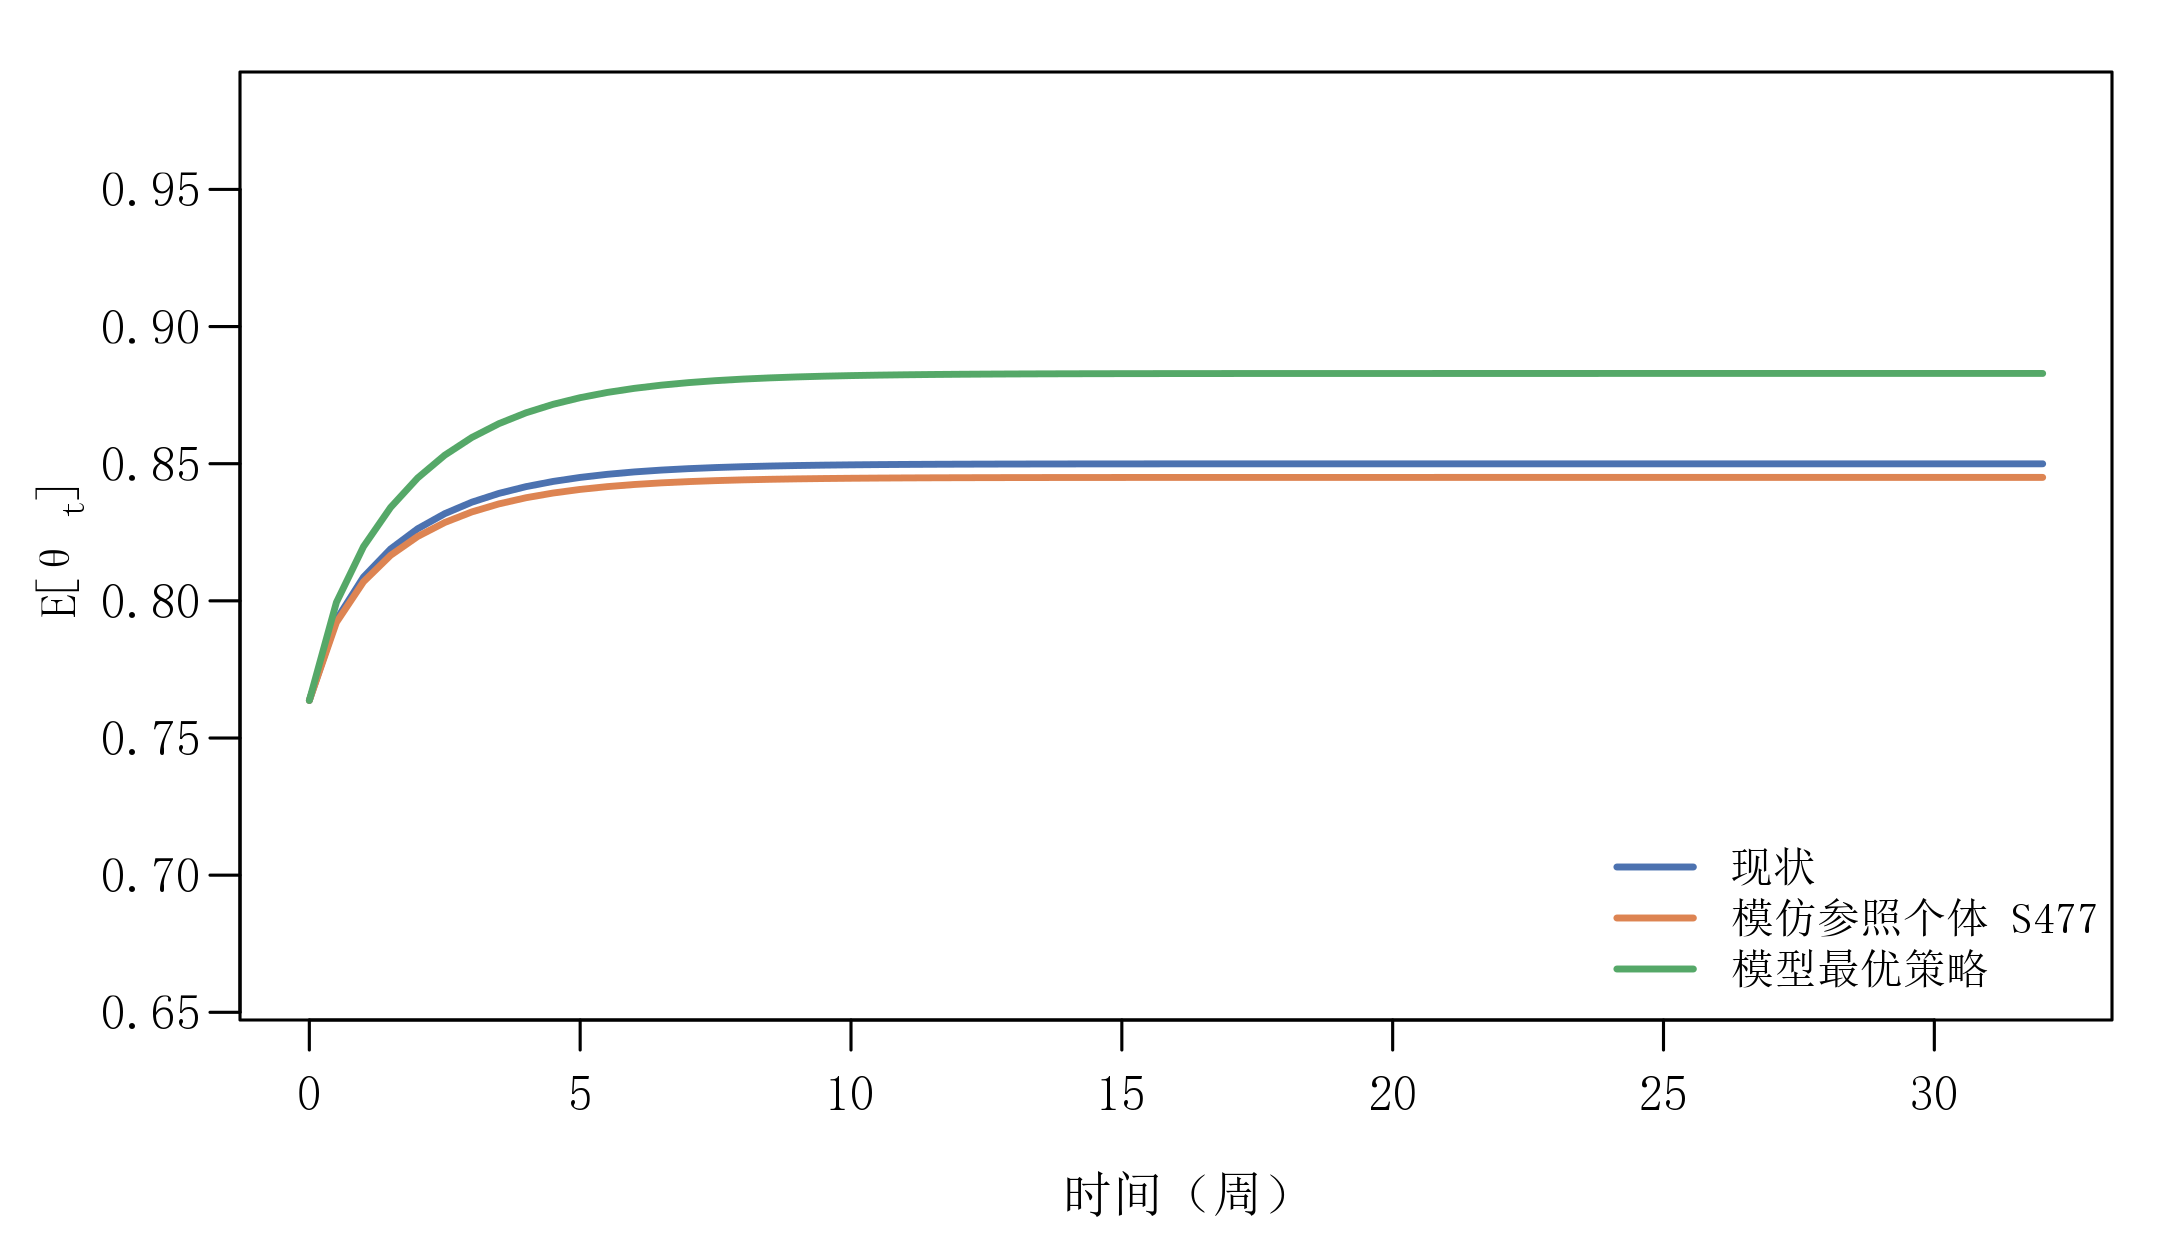
\includegraphics[width=0.85\textwidth]{fig_gain}
\caption{三种方案下的期望效率轨迹 $\E[\theta_t]$（0—32 周）}
\label{fig:gain}
\end{figure}

\begin{figure}[H]
\centering
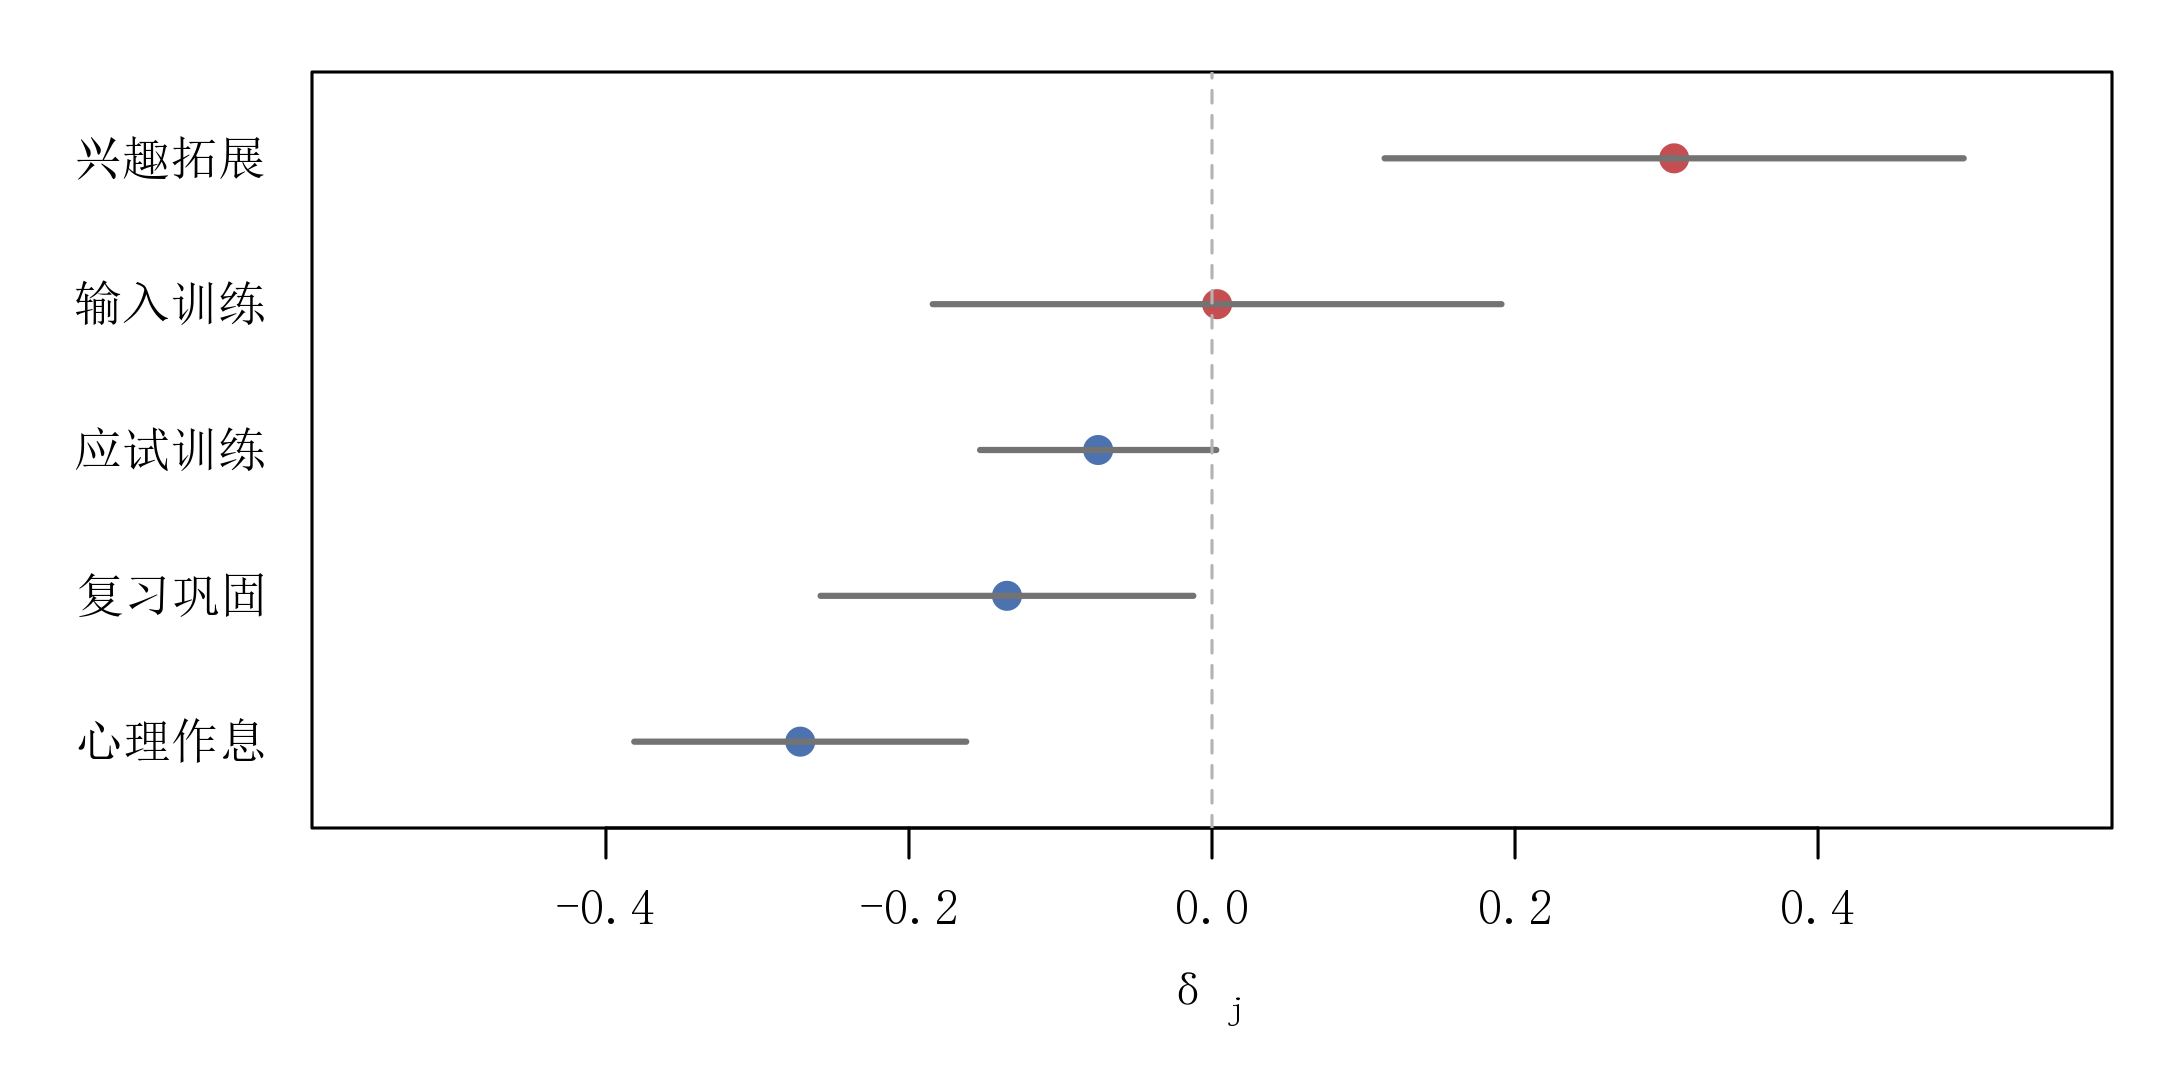
\includegraphics[width=0.85\textwidth]{fig_strategy}
\caption{五个协变量的行为杠杆效应 $\delta_j$ 及 95\% 置信区间}
\label{fig:strategy}
\end{figure}

\begin{figure}[H]
\centering
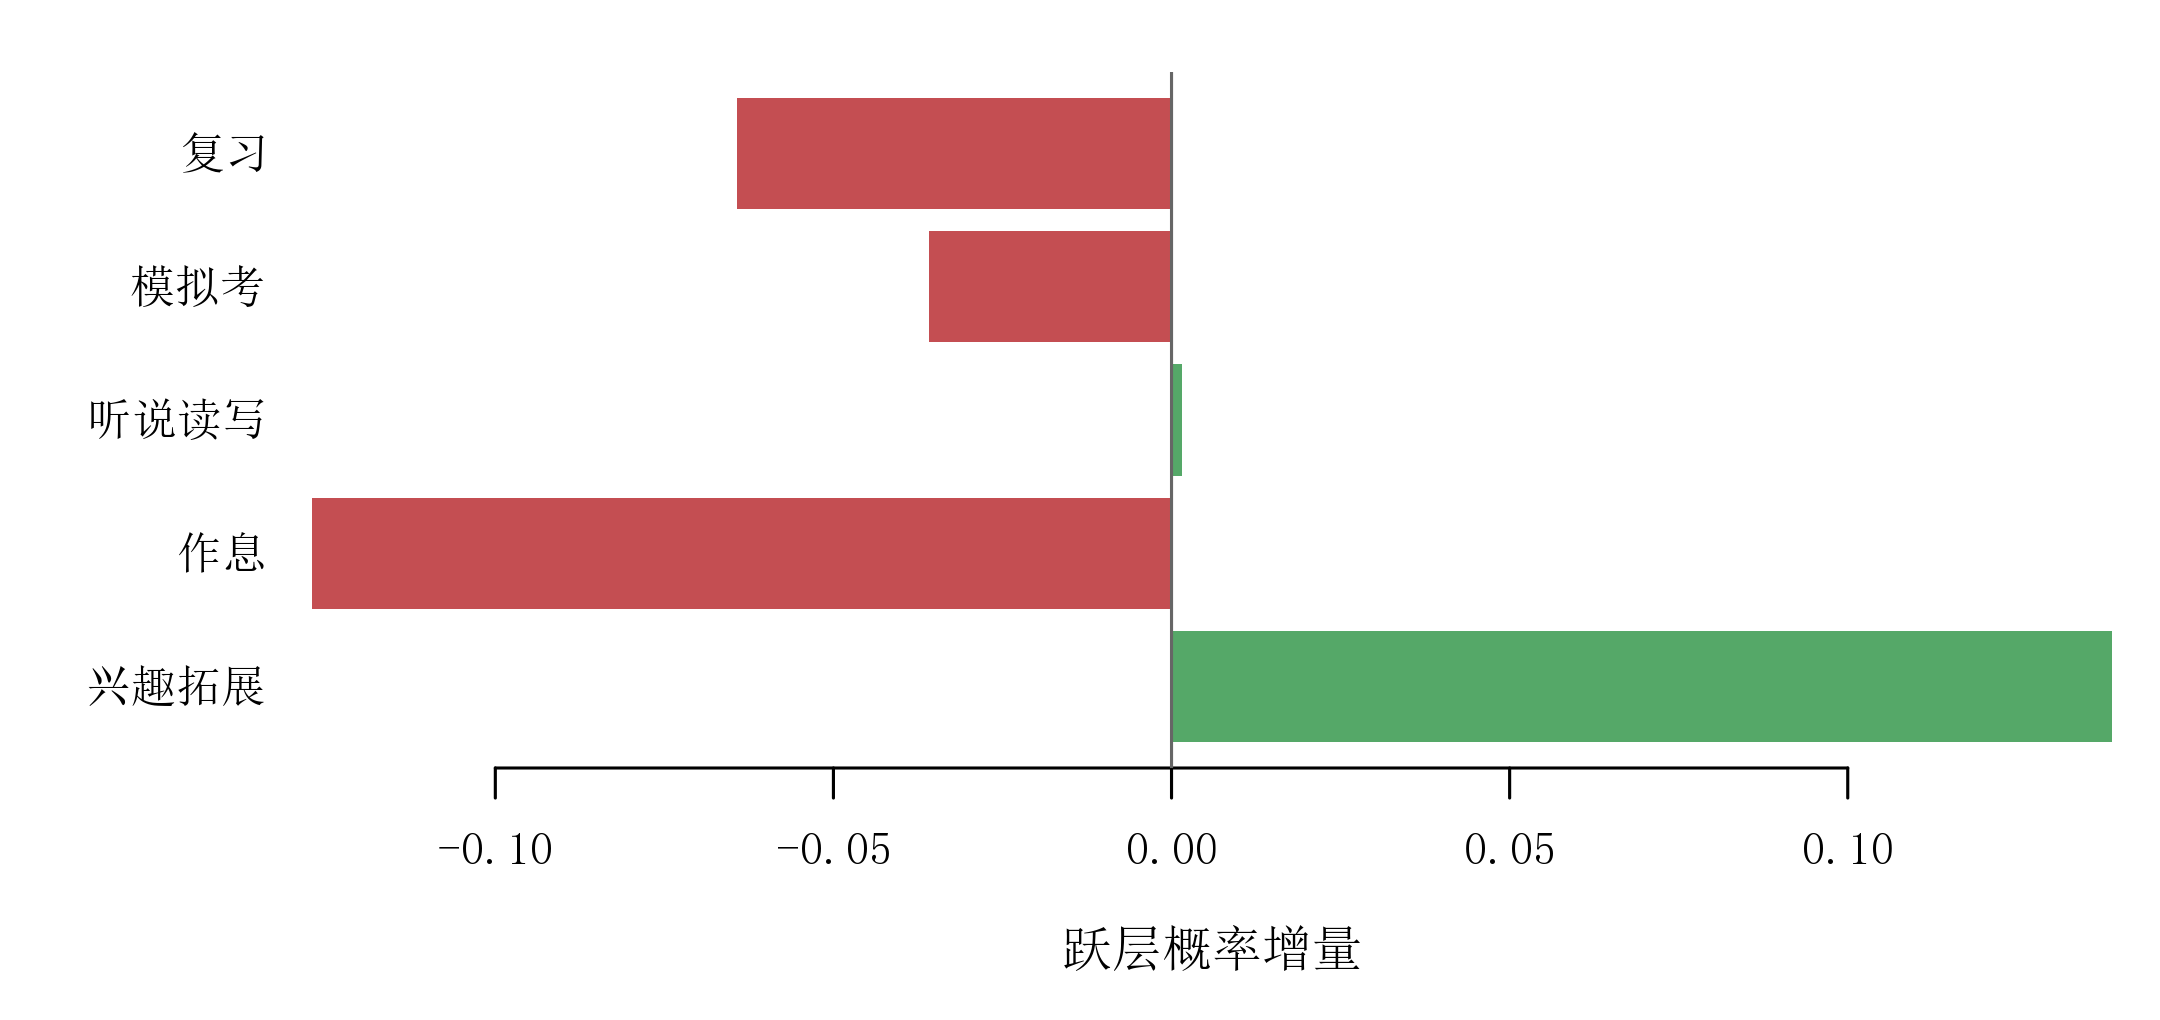
\includegraphics[width=0.85\textwidth]{fig_action}
\caption{S480 单独实施每个动作后的 16 周跃层概率增量（相对现状）}
\label{fig:action}
\end{figure}

图 \ref{fig:strategy} 把 $\delta_j$ 的符号与置信区间摆在一起：只有“兴趣
拓展”的区间整体位于 0 的右侧，“心理作息”的区间整体位于左侧，其余三项跨
越 0。这一图形化的结果比表 \ref{tab:ctmcpar} 更直观地说明“哪一个杠杆真的
有效”。图 \ref{fig:action} 则显示：单独实施“兴趣拓展”可使跃层概率提高约
0.10，单独实施“作息改善”会使其下降约 0.10，其余动作的影响在 $\pm0.05$ 以
内。两张图合起来回答了一个原文回答不了的问题：\textbf{在有限学时下，应当
先动哪一个维度}。

\subsubsection{小结：随机过程给出的四类新信息}

把本节的结果与原文对照，随机过程至少补上了四类原文没有的信息：

\begin{enumerate}[label=（\arabic*）,itemsep=2pt,topsep=2pt,leftmargin=3em]
\item \textbf{方向}：$\rho_i$ 的符号与大小，回答“这个人会自己变好还是变
  坏”。98.1\% 的 $\rho_i<1$ 说明“下行锁定”是群体性现象，而不是个别现象。
\item \textbf{概率}：$\bP_i(t)$ 给出任意时长内的跃层概率，把“能不能上去”
  从定性判断变成可计算的数值。
\item \textbf{时间}：$m_k$ 与 $T(43.97\%)$ 给出“多久”，把“一学期”“三学
  期”这样的模糊表述换成周。
\item \textbf{策略}：式\eqref{eq:opt} 给出“做什么、做多少”，并用 $\delta$
  的符号筛掉“看起来努力、实际稀释效率”的动作。
\end{enumerate}







